\documentclass{standalone}
\usepackage{tikz}
\usetikzlibrary{patterns, positioning}
\usepackage[sfdefault]{ClearSans} %% option 'sfdefault' activates Clear Sans as the default text font
\usepackage[T1]{fontenc}

\begin{document}
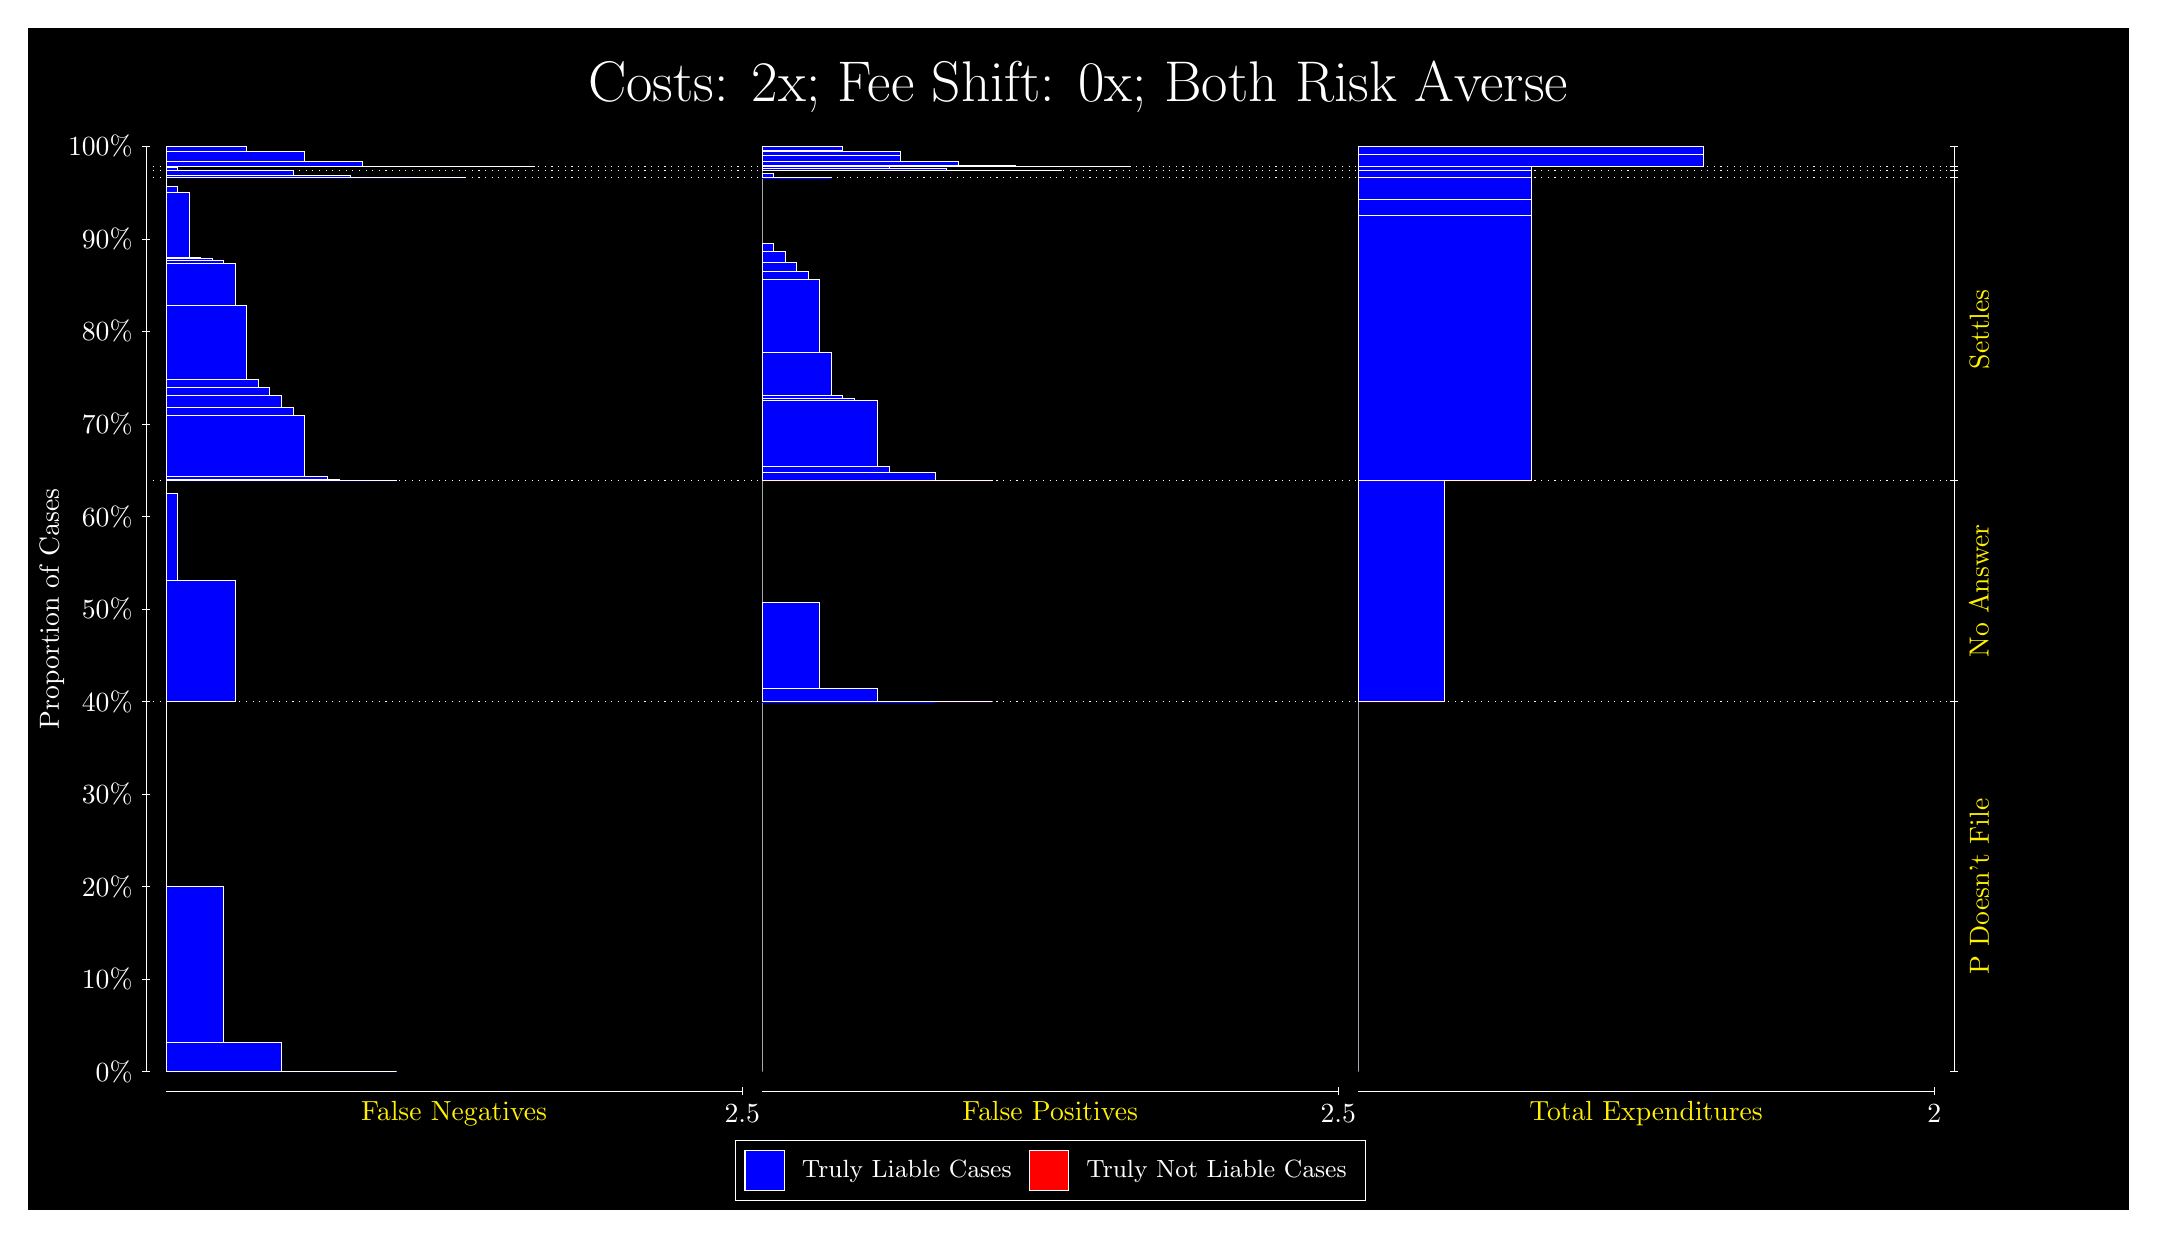
\begin{tikzpicture}
\draw[fill=black] (0,0) rectangle (26.667,15);
\draw[text=white] (0,13.5) rectangle (26.667,15) node[midway] {\huge Costs: 2x; Fee Shift: 0x; Both Risk Averse};
\draw[white, very thin] (1.5,1.75) -- (1.5,13.5);
\node[rotate=90, text=white, anchor=center] at (0.3, 7.625) {Proportion of Cases};
\draw[white, very thin] (1.45,1.75) -- (1.55,1.75);
\node[text=white, anchor=east] at (1.45, 1.75) {0\%};
\draw[white, very thin] (1.45,2.925) -- (1.55,2.925);
\node[text=white, anchor=east] at (1.45, 2.925) {10\%};
\draw[white, very thin] (1.45,4.1) -- (1.55,4.1);
\node[text=white, anchor=east] at (1.45, 4.1) {20\%};
\draw[white, very thin] (1.45,5.275) -- (1.55,5.275);
\node[text=white, anchor=east] at (1.45, 5.275) {30\%};
\draw[white, very thin] (1.45,6.45) -- (1.55,6.45);
\node[text=white, anchor=east] at (1.45, 6.45) {40\%};
\draw[white, very thin] (1.45,7.625) -- (1.55,7.625);
\node[text=white, anchor=east] at (1.45, 7.625) {50\%};
\draw[white, very thin] (1.45,8.8) -- (1.55,8.8);
\node[text=white, anchor=east] at (1.45, 8.8) {60\%};
\draw[white, very thin] (1.45,9.975) -- (1.55,9.975);
\node[text=white, anchor=east] at (1.45, 9.975) {70\%};
\draw[white, very thin] (1.45,11.15) -- (1.55,11.15);
\node[text=white, anchor=east] at (1.45, 11.15) {80\%};
\draw[white, very thin] (1.45,12.325) -- (1.55,12.325);
\node[text=white, anchor=east] at (1.45, 12.325) {90\%};
\draw[white, very thin] (1.45,13.5) -- (1.55,13.5);
\node[text=white, anchor=east] at (1.45, 13.5) {100\%};

\draw[white, very thin] (24.457,1.75) -- (24.457,13.5);
\draw[white, very thin] (24.407,1.75) -- (24.507,1.75);
\node[anchor=west] at (24.407, 1.75) {};
\draw[white, very thin] (24.407,6.4489) -- (24.507,6.4489);
\node[anchor=west] at (24.407, 6.4489) {};
\draw[white, very thin] (24.407,9.2559) -- (24.507,9.2559);
\node[anchor=west] at (24.407, 9.2559) {};
\draw[white, very thin] (24.407,13.101) -- (24.507,13.101);
\node[anchor=west] at (24.407, 13.101) {};
\draw[white, very thin] (24.407,13.197) -- (24.507,13.197);
\node[anchor=west] at (24.407, 13.197) {};
\draw[white, very thin] (24.407,13.248) -- (24.507,13.248);
\node[anchor=west] at (24.407, 13.248) {};
\draw[white, very thin] (24.407,13.5) -- (24.507,13.5);
\node[anchor=west] at (24.407, 13.5) {};

\draw[white, very thin, fill=blue] (1.75,1.75) rectangle (4.6775,1.75);
\draw[white, very thin, fill=blue] (1.75,1.75) rectangle (3.9457,1.7532);
\draw[white, very thin, fill=blue] (1.75,1.7532) rectangle (3.2138,2.126);
\draw[white, very thin, fill=blue] (1.75,2.126) rectangle (2.4819,4.1027);
\draw[white, very thin, fill=red] (1.75,4.1027) rectangle (1.75,4.1027);
\draw[white, very thin, fill=blue] (1.75,4.1027) rectangle (1.75,6.4489);
\draw[white, very thin, fill=blue] (1.75,6.4489) rectangle (2.6283,7.9892);
\draw[white, very thin, fill=blue] (1.75,7.9892) rectangle (1.8964,9.0897);
\draw[white, very thin, fill=red] (1.75,9.0897) rectangle (1.75,9.0897);
\draw[white, very thin, fill=blue] (1.75,9.0897) rectangle (1.75,9.2559);
\draw[white, very thin, fill=blue] (1.75,9.2559) rectangle (4.6775,9.256);
\draw[white, very thin, fill=blue] (1.75,9.256) rectangle (4.3848,9.256);
\draw[white, very thin, fill=blue] (1.75,9.256) rectangle (4.092,9.2562);
\draw[white, very thin, fill=blue] (1.75,9.2562) rectangle (3.9457,9.2768);
\draw[white, very thin, fill=blue] (1.75,9.2768) rectangle (3.7993,9.3034);
\draw[white, very thin, fill=blue] (1.75,9.3034) rectangle (3.6529,9.3087);
\draw[white, very thin, fill=blue] (1.75,9.3087) rectangle (3.5065,10.09);
\draw[white, very thin, fill=blue] (1.75,10.09) rectangle (3.3602,10.187);
\draw[white, very thin, fill=blue] (1.75,10.187) rectangle (3.2138,10.334);
\draw[white, very thin, fill=blue] (1.75,10.334) rectangle (3.0674,10.443);
\draw[white, very thin, fill=blue] (1.75,10.443) rectangle (2.921,10.543);
\draw[white, very thin, fill=blue] (1.75,10.543) rectangle (2.7746,11.476);
\draw[white, very thin, fill=blue] (1.75,11.476) rectangle (2.6283,12.02);
\draw[white, very thin, fill=blue] (1.75,12.02) rectangle (2.4819,12.055);
\draw[white, very thin, fill=blue] (1.75,12.055) rectangle (2.3355,12.082);
\draw[white, very thin, fill=blue] (1.75,12.082) rectangle (2.1891,12.087);
\draw[white, very thin, fill=blue] (1.75,12.087) rectangle (2.0428,12.915);
\draw[white, very thin, fill=blue] (1.75,12.915) rectangle (1.8964,12.997);
\draw[white, very thin, fill=red] (1.75,12.997) rectangle (1.75,12.997);
\draw[white, very thin, fill=blue] (1.75,12.997) rectangle (1.75,13.101);
\draw[white, very thin, fill=blue] (1.75,13.101) rectangle (5.5558,13.101);
\draw[white, very thin, fill=blue] (1.75,13.101) rectangle (4.8239,13.101);
\draw[white, very thin, fill=blue] (1.75,13.101) rectangle (4.092,13.137);
\draw[white, very thin, fill=blue] (1.75,13.137) rectangle (3.3602,13.196);
\draw[white, very thin, fill=blue] (1.75,13.196) rectangle (2.6283,13.197);
\draw[white, very thin, fill=red] (1.75,13.197) rectangle (1.75,13.197);
\draw[white, very thin, fill=blue] (1.75,13.197) rectangle (2.6283,13.198);
\draw[white, very thin, fill=blue] (1.75,13.198) rectangle (1.8964,13.229);
\draw[white, very thin, fill=red] (1.75,13.229) rectangle (1.75,13.229);
\draw[white, very thin, fill=blue] (1.75,13.229) rectangle (1.75,13.248);
\draw[white, very thin, fill=blue] (1.75,13.248) rectangle (6.4341,13.248);
\draw[white, very thin, fill=blue] (1.75,13.248) rectangle (5.7022,13.248);
\draw[white, very thin, fill=blue] (1.75,13.248) rectangle (4.9703,13.252);
\draw[white, very thin, fill=blue] (1.75,13.252) rectangle (4.2384,13.31);
\draw[white, very thin, fill=blue] (1.75,13.31) rectangle (3.5065,13.437);
\draw[white, very thin, fill=blue] (1.75,13.437) rectangle (2.7746,13.495);
\draw[white, very thin, fill=blue] (1.75,13.495) rectangle (2.0428,13.5);
\draw[white, very thin, fill=red] (1.75,13.5) rectangle (1.75,13.5);
\draw[white, very thin, fill=blue] (1.75,13.5) rectangle (1.75,13.5);
\draw[white, very thin, fill=red] (9.3189,1.75) rectangle (9.3189,1.75);
\draw[white, very thin, fill=blue] (9.3189,1.75) rectangle (9.3189,6.4489);
\draw[white, very thin, fill=red] (9.3189,6.4489) rectangle (12.246,6.4489);
\draw[white, very thin, fill=blue] (9.3189,6.4489) rectangle (12.246,6.4489);
\draw[white, very thin, fill=blue] (9.3189,6.4489) rectangle (11.515,6.4492);
\draw[white, very thin, fill=blue] (9.3189,6.4492) rectangle (10.783,6.6152);
\draw[white, very thin, fill=blue] (9.3189,6.6152) rectangle (10.051,7.7157);
\draw[white, very thin, fill=blue] (9.3189,7.7157) rectangle (9.3189,9.2559);
\draw[white, very thin, fill=red] (9.3189,9.2559) rectangle (12.246,9.2559);
\draw[white, very thin, fill=blue] (9.3189,9.2559) rectangle (12.246,9.2562);
\draw[white, very thin, fill=red] (9.3189,9.2562) rectangle (11.954,9.2562);
\draw[white, very thin, fill=blue] (9.3189,9.2562) rectangle (11.954,9.2562);
\draw[white, very thin, fill=red] (9.3189,9.2562) rectangle (11.661,9.2562);
\draw[white, very thin, fill=blue] (9.3189,9.2562) rectangle (11.661,9.2563);
\draw[white, very thin, fill=blue] (9.3189,9.2563) rectangle (11.515,9.3596);
\draw[white, very thin, fill=red] (9.3189,9.3596) rectangle (11.368,9.3596);
\draw[white, very thin, fill=blue] (9.3189,9.3596) rectangle (11.368,9.3596);
\draw[white, very thin, fill=blue] (9.3189,9.3596) rectangle (11.222,9.3596);
\draw[white, very thin, fill=red] (9.3189,9.3596) rectangle (11.075,9.3596);
\draw[white, very thin, fill=blue] (9.3189,9.3596) rectangle (11.075,9.3597);
\draw[white, very thin, fill=blue] (9.3189,9.3597) rectangle (10.929,9.442);
\draw[white, very thin, fill=blue] (9.3189,9.442) rectangle (10.783,10.27);
\draw[white, very thin, fill=blue] (9.3189,10.27) rectangle (10.636,10.275);
\draw[white, very thin, fill=blue] (9.3189,10.275) rectangle (10.49,10.302);
\draw[white, very thin, fill=blue] (9.3189,10.302) rectangle (10.344,10.337);
\draw[white, very thin, fill=blue] (9.3189,10.337) rectangle (10.197,10.881);
\draw[white, very thin, fill=blue] (9.3189,10.881) rectangle (10.051,11.814);
\draw[white, very thin, fill=blue] (9.3189,11.814) rectangle (9.9044,11.913);
\draw[white, very thin, fill=blue] (9.3189,11.913) rectangle (9.758,12.023);
\draw[white, very thin, fill=blue] (9.3189,12.023) rectangle (9.6116,12.17);
\draw[white, very thin, fill=blue] (9.3189,12.17) rectangle (9.4652,12.267);
\draw[white, very thin, fill=blue] (9.3189,12.267) rectangle (9.3189,13.101);
\draw[white, very thin, fill=red] (9.3189,13.101) rectangle (10.197,13.101);
\draw[white, very thin, fill=blue] (9.3189,13.101) rectangle (10.197,13.102);
\draw[white, very thin, fill=blue] (9.3189,13.102) rectangle (9.4652,13.161);
\draw[white, very thin, fill=blue] (9.3189,13.161) rectangle (9.3189,13.197);
\draw[white, very thin, fill=red] (9.3189,13.197) rectangle (13.125,13.197);
\draw[white, very thin, fill=blue] (9.3189,13.197) rectangle (13.125,13.197);
\draw[white, very thin, fill=blue] (9.3189,13.197) rectangle (12.393,13.197);
\draw[white, very thin, fill=blue] (9.3189,13.197) rectangle (11.661,13.216);
\draw[white, very thin, fill=blue] (9.3189,13.216) rectangle (10.929,13.247);
\draw[white, very thin, fill=blue] (9.3189,13.247) rectangle (10.197,13.248);
\draw[white, very thin, fill=red] (9.3189,13.248) rectangle (14.003,13.248);
\draw[white, very thin, fill=blue] (9.3189,13.248) rectangle (14.003,13.248);
\draw[white, very thin, fill=red] (9.3189,13.248) rectangle (13.271,13.248);
\draw[white, very thin, fill=blue] (9.3189,13.248) rectangle (13.271,13.248);
\draw[white, very thin, fill=red] (9.3189,13.248) rectangle (12.539,13.248);
\draw[white, very thin, fill=blue] (9.3189,13.248) rectangle (12.539,13.253);
\draw[white, very thin, fill=blue] (9.3189,13.253) rectangle (11.807,13.311);
\draw[white, very thin, fill=red] (9.3189,13.311) rectangle (11.807,13.311);
\draw[white, very thin, fill=blue] (9.3189,13.311) rectangle (11.807,13.311);
\draw[white, very thin, fill=blue] (9.3189,13.311) rectangle (11.075,13.392);
\draw[white, very thin, fill=red] (9.3189,13.392) rectangle (11.075,13.392);
\draw[white, very thin, fill=blue] (9.3189,13.392) rectangle (11.075,13.438);
\draw[white, very thin, fill=blue] (9.3189,13.438) rectangle (10.344,13.45);
\draw[white, very thin, fill=blue] (9.3189,13.45) rectangle (10.344,13.496);
\draw[white, very thin, fill=blue] (9.3189,13.496) rectangle (9.6116,13.496);
\draw[white, very thin, fill=blue] (9.3189,13.496) rectangle (9.6116,13.5);
\draw[white, very thin, fill=blue] (9.3189,13.5) rectangle (9.3189,13.5);
\draw[white, very thin, fill=red] (16.888,1.75) rectangle (16.888,1.75);
\draw[white, very thin, fill=blue] (16.888,1.75) rectangle (16.888,6.4489);
\draw[white, very thin, fill=red] (16.888,6.4489) rectangle (17.986,6.4489);
\draw[white, very thin, fill=blue] (16.888,6.4489) rectangle (17.986,9.2559);
\draw[white, very thin, fill=red] (16.888,9.2559) rectangle (19.083,9.2559);
\draw[white, very thin, fill=blue] (16.888,9.2559) rectangle (19.083,12.625);
\draw[white, very thin, fill=red] (16.888,12.625) rectangle (19.083,12.625);
\draw[white, very thin, fill=blue] (16.888,12.625) rectangle (19.083,12.828);
\draw[white, very thin, fill=red] (16.888,12.828) rectangle (19.083,12.828);
\draw[white, very thin, fill=blue] (16.888,12.828) rectangle (19.083,13.101);
\draw[white, very thin, fill=red] (16.888,13.101) rectangle (19.083,13.101);
\draw[white, very thin, fill=blue] (16.888,13.101) rectangle (19.083,13.197);
\draw[white, very thin, fill=red] (16.888,13.197) rectangle (19.083,13.197);
\draw[white, very thin, fill=blue] (16.888,13.197) rectangle (19.083,13.248);
\draw[white, very thin, fill=red] (16.888,13.248) rectangle (21.279,13.248);
\draw[white, very thin, fill=blue] (16.888,13.248) rectangle (21.279,13.404);
\draw[white, very thin, fill=red] (16.888,13.404) rectangle (21.279,13.404);
\draw[white, very thin, fill=blue] (16.888,13.404) rectangle (21.279,13.5);
\draw[white, dotted] (1.5,6.4489) -- (24.457,6.4489);
\draw[white, dotted] (1.5,9.2559) -- (24.457,9.2559);
\draw[white, dotted] (1.5,13.101) -- (24.457,13.101);
\draw[white, dotted] (1.5,13.197) -- (24.457,13.197);
\draw[white, dotted] (1.5,13.248) -- (24.457,13.248);
\draw[white, very thin] (1.75,1.5) -- (9.0689,1.5);
\node[text=yellow, anchor=north] at (5.4094, 1.5) {False Negatives};
\draw[white, very thin] (9.0689,1.45) -- (9.0689,1.55);
\node[text=white, anchor=north] at (9.0689, 1.45) {2.5};

\draw[white, very thin] (9.3189,1.5) -- (16.638,1.5);
\node[text=yellow, anchor=north] at (12.978, 1.5) {False Positives};
\draw[white, very thin] (16.638,1.45) -- (16.638,1.55);
\node[text=white, anchor=north] at (16.638, 1.45) {2.5};

\draw[white, very thin] (16.888,1.5) -- (24.207,1.5);
\node[text=yellow, anchor=north] at (20.547, 1.5) {Total Expenditures};
\draw[white, very thin] (24.207,1.45) -- (24.207,1.55);
\node[text=white, anchor=north] at (24.207, 1.45) {2};

\node[text=yellow, centered, rotate=90] at (24.777, 4.0995) {P Doesn't File};
\node[text=yellow, centered, rotate=90] at (24.777, 7.8524) {No Answer};
\node[text=yellow, centered, rotate=90] at (24.777, 11.178) {Settles};




\draw (12.978300999999998,1.5) node[draw=none] (baseCoordinate) {};
\begin{scope}[align=center]
        \matrix[scale=0.5, draw=white, below=0.5cm of baseCoordinate, nodes={draw}, column sep=0.1cm]{
            \node[rectangle, draw, minimum width=0.5cm, minimum height=0.5cm, fill=blue] {}; &
            \node[draw=none, font=\small, text=white] (B) {Truly Liable Cases}; &
            \node[rectangle, draw, minimum width=0.5cm, minimum height=0.5cm, fill=red] {}; &
            \node[draw=none, font=\small, text=white] (B) {Truly Not Liable Cases}; \\
            };
\end{scope}

\end{tikzpicture}
\end{document}